\section{One compiler, seven constraint types}\label{sec:validation}
All experiments use one code path: constraint set $\to$ automaton $\to$ $A_q$ (numerically and as a Qiskit circuit) $\to$ amplitude amplification and QAOA. The automaton is built from the truth table for $n\le16$ and, for larger instances, written from the problem structure. The families are cardinality with a quadratic risk objective, knapsack with different weights, weighted independent set, set packing, exact cover, $3$-colouring and quadratic assignment, with five random instances each (tables in \cref{sec:pipeline}).

\begin{figure*}[t]\centering
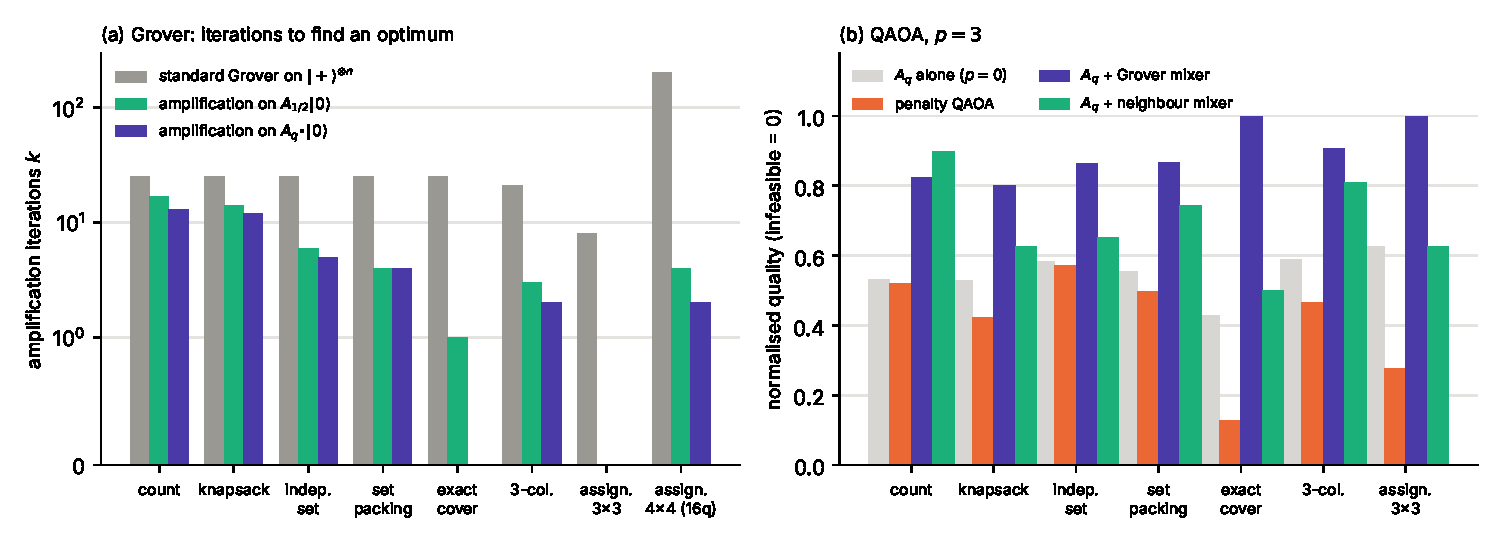
\includegraphics[width=\textwidth]{figures/fig_general.pdf}
\caption{\orig{exact ideal numerics} One pipeline on seven constraint types. (a) Amplification iterations to find an optimum: standard Grover, $A_{1/2}$, and $A_q$ with the best bias (symmetric log axis); a missing bar is $k=0$, i.e.\ measuring $A_q|0\rangle$ already finds an optimum with high probability. (b) QAOA at $p=3$: quality, infeasible samples counted as $0$.}\label{fig:general}
\end{figure*}

\paragraph{Amplification.} The gain follows the tightness of the constraint. With loose constraints (cardinality, knapsack; $|F|/2^n\approx0.2$--$0.4$) the saving is $1.5$--$2\times$ ($25\to17$ and $25\to14$ iterations at $q=\tfrac12$). With tight constraints it is large: independent set $25\to6$, set packing $25\to4$, $3$-colouring $21\to3$, exact cover $25\to1$; for $3\times3$ assignments the optimum is found by measuring $A_q|0\rangle$, and for $4\times4$ permutations ($24$ feasible strings among $65\,536$) standard Grover needs $201$ iterations and $A_q$ needs $4$ ($2$ with the best bias).

\paragraph{QAOA.} With the Grover mixer every sample is feasible, at every depth and for arbitrary angles (the smallest feasible mass over all instances, depths and methods is $1-3\cdot10^{-16}$). Penalty QAOA, with the best of four penalty weights, has $21$--$95\,\%$ feasible samples, falling with the tightness, and a lower quality on all seven families; at $p=3$ the Grover mixer wins in quality on $34$ of $34$ instances (median $0.80$--$1.00$ against $0.13$--$0.57$). For the $4\times4$ assignment penalty QAOA gives $2.6\,\%$ feasible samples and quality $0.014$, against $100\,\%$ and $0.82$ for $A_q$. Two caveats: exact cover and assignment have only $3$--$6$ feasible strings, so they show the mechanism and not difficulty; and local mixers need a connected move graph (the neighbour mixer does not move the state on exact cover and permutations), so cheap mixers are structure-dependent while the Grover mixer is general at the price of two copies of $A_q$ per layer.

\paragraph{Circuits and scale.} The compiled circuits reproduce the exact formulas to $8\cdot10^{-15}$ (all Grover iterations) and $5\cdot10^{-16}$ ($p=2$ QAOA); the compiled $A_q$ costs $24$--$297$ CZ gates for the six $n=6$ families, without hand optimisation. With the automaton written from the structure of the problem, the same compiler runs on matrix-product states up to $60$ variables for a cardinality constraint ($274$ qubits), $80$ for a band independent set ($236$) and $30$ for knapsack ($145$); all $15$ instances ($7$ configurations) give $100\,\%$ feasible shots against uniform feasible shares down to $2\cdot10^{-11}$. These runs validate the circuits at scale and say nothing about advantage.

\paragraph{Where it fails.} Market split ($m$ equalities on random integers) is the opposite case: exact look-ahead would solve the instance, and the practical bound-only relaxation has width $21$ at $n=10$ and $12\,067$ at $n=20$, while the iterations shrink only fourfold. There the circuit grows faster than the iterations shrink and the construction does not pay. The width--completeness dial is monotone and sound: tracking a knapsack weight only up to a lower bound reduces the width from $33$ to $1$, and the iterations rise from $25$ to the $50$ of standard Grover (\cref{prop:relax}).
